\documentclass[11pt,twocolumn]{article}
\usepackage{geometry}                % See geometry.pdf to learn the layout options. There are lots.
\geometry{letterpaper}                   % ... or a4paper or a5paper or ... 
%\geometry{landscape}                % Activate for for rotated page geometry
%\usepackage[parfill]{parskip}    % Activate to begin paragraphs with an empty line rather than an indent
\usepackage{graphicx}
\usepackage{amssymb}
\usepackage{subfigure}
\usepackage{epstopdf}
\usepackage{cite}
\usepackage{url}
\DeclareGraphicsRule{.tif}{png}{.png}{`convert #1 `dirname #1`/`basename #1 .tif`.png}

\title{Modeling the Wireless Channel from Empirical Data}
\author{Kok-Kiong Yap}
%\date{}                                           % Activate to display a given date or no date

\begin{document}
\maketitle

\begin{abstract}
Unlike previous simulators, which strives to abstract and model the various features of the wireless channel, we present a different approach of model the channel via its statistics.  This document outlines the extraction of an approximation for path loss attenuation in a wireless channel from empirical experiments.  It also presents how the data can be used to model the channel in simulation.
\end{abstract}

\section{Motivation}
While the wireless channel is much studied over the last few decades, much difficulty continues to plague the networking simulation.  An accurate model of the wireless channel invariantly creates a simulation that will takes large amount of memory and/or time.  Meanwhile, an inaccurate model casts doubts on the validity of the results.   Previous simulators have strived to abstract and model the various features of the wireless channel \cite{ns2}.

Here, we take a different approach by modeling the wireless channel directly from experimental measurement.  Specifically, the data used to model the wireless channel is from \cite{roofnetdata}, specifically the data probe done from May 2004 to August 2004.  The content of this is related to \cite{Aguayo:2004lr}, from the people who have kindly shared these data.

\section{Reception Probabilities}
In networking simulation, a useful characteristic to map is the reception percentage, which is proportional to the probabilities of reception or error.  We distill the average reception percentage of all node pairs form the data and plot them in scatter plots presented in Fig.~\ref{fig:scatter}.  The following $5$ cases are being considered here.
\begin{enumerate}
\item Short packet of $60$ bytes payload at rate of $1$ $Mbps$
\item Long packet of $1500$ bytes payload at rate of $1$ $Mbps$
\item Long packet of $1500$ bytes payload at rate of $2$ $Mbps$
\item Long packet of $1500$ bytes payload at rate of $5.5$ $Mbps$
\item Long packet of $1500$ bytes payload at rate of $11$ $Mbps$
\end{enumerate}

\begin{figure*}
\centering
\mbox{\subfigure[$1$ Mbps, Short Packet]{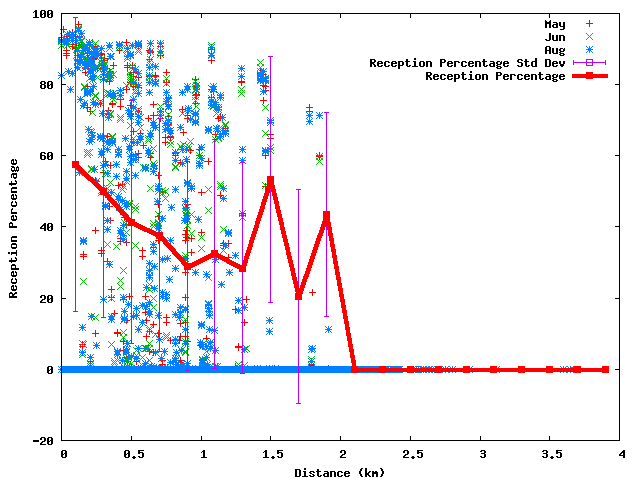
\includegraphics[width=0.5\linewidth]{DistroScatterPlot1}}
\subfigure[$1$ Mbps, Long Packet]{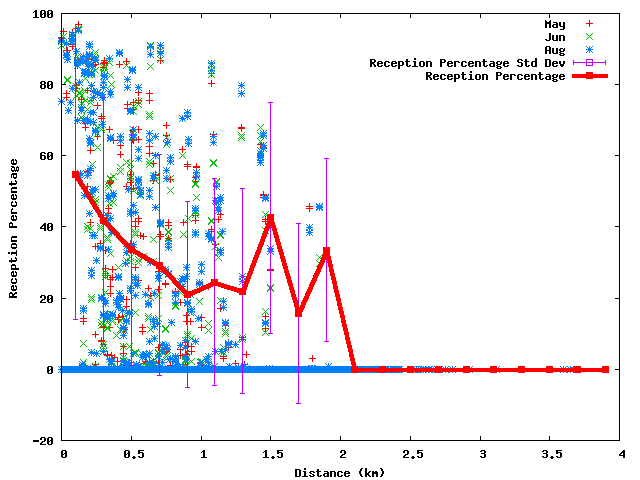
\includegraphics[width=0.5\linewidth]{DistroScatterPlot2}}}
\mbox{\subfigure[$2$ Mbps, Long Packet]{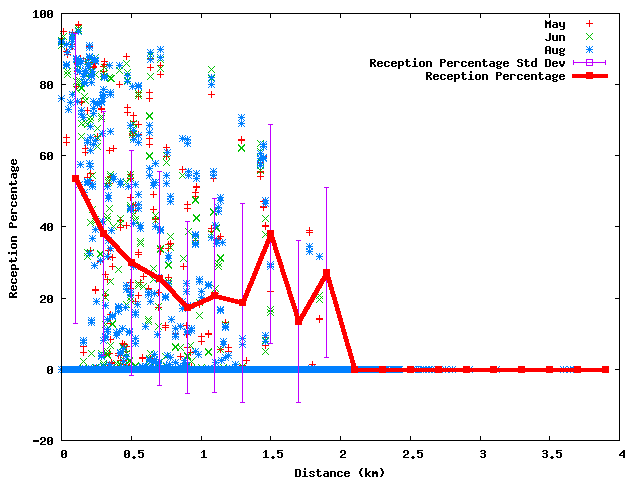
\includegraphics[width=0.5\linewidth]{DistroScatterPlot3}}
\subfigure[$5.5$ Mbps, Long Packet]{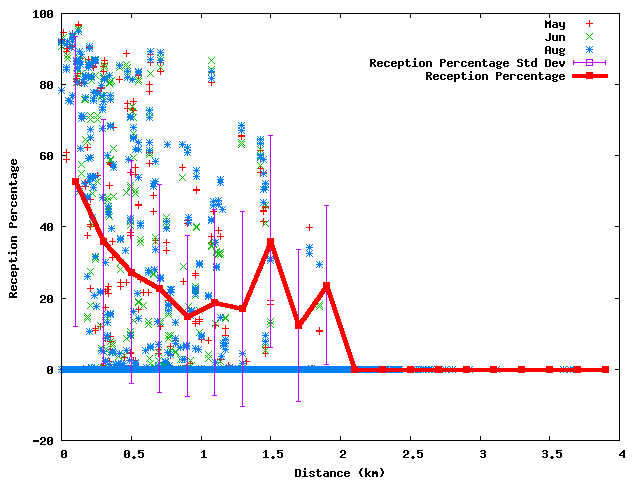
\includegraphics[width=0.5\linewidth]{DistroScatterPlot4}}}
\subfigure[$11$ Mbps, Long Packet]{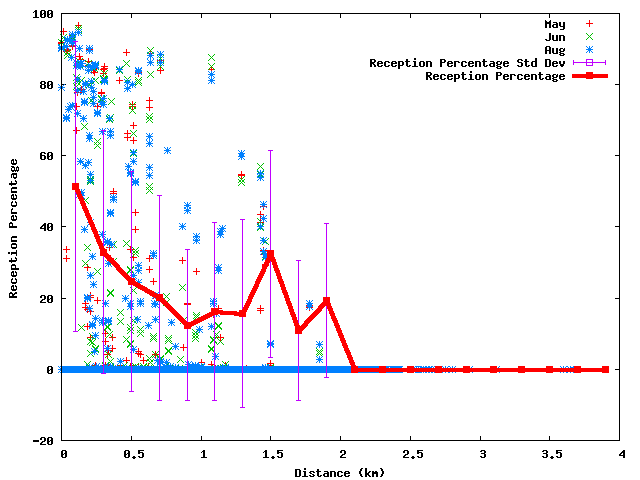
\includegraphics[width=0.5\linewidth]{DistroScatterPlot5}}
\caption{Plots of reception probability across distance, with scatter plots of the various node pairs in the RoofNet system.}
\label{fig:scatter}
\end{figure*}

We then divide the distance from $0$ to $4$ $km$ into $20$ bins, and consider the distribution of reception percentage within each bin.  The bin size is chosen for most bins to have significant number of samples to give the mean and standard deviation.  The mean and standard deviation of the distribution within each bin is also being presented in Fig.~\ref{fig:scatter}.  We have also collated the different cases in Fig.~\ref{fig:prob}.  

\begin{figure*}[ht]
\centering
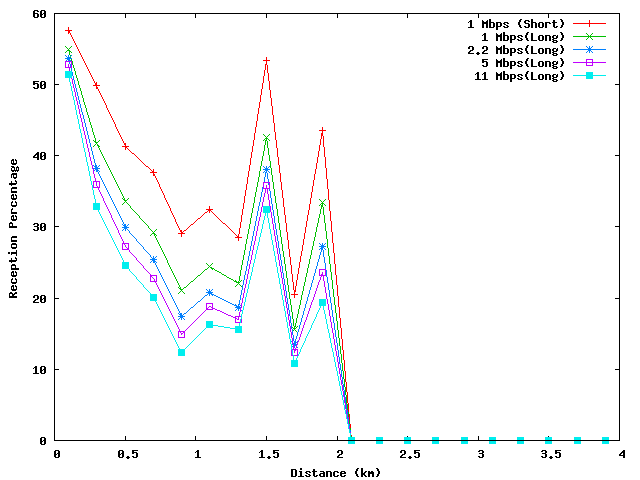
\includegraphics[width=0.8\linewidth]{Distro}
\caption{Expected reception percentage as a function of distance}
\label{fig:prob}
\end{figure*}

As we can observe, the commonly assumed monotonically decreasing reception probabilities does not hold in this case.  The peaks are around $1.5$ and $1.9$ $km$ are surprising and is likely to be environment specific.  Note that this profile is observed over all five cases.  Nevertheless, this is a possible operating environment for Wi-Fi networks, which we have to consider.

We also notice that increasing the size of the packet and/or the rate does indeed lowers the reception percentage.  This result is intuitive and natural, especially since the profile is being maintained across all the cases.  We also note that there is no reception beyond $2.1$ $km$.

\section{\textit{Caveat emptor}}
\subsection{Data Availability}
From the data downloaded from \cite{roofnetdata}, it appears that the file recording reception probabilities of some node pairs are not available.  Meanwhile, there are pairs that have empty files, i.e., does not generate any data.  We assume that the absence of a file means that the channel is not being measured and thus excluded from the tabulations; while the presence of an empty signifies zero reception probabilities.

It should be mentioned that if we include all node pairs regardless of the presence of files, we will have reception probabilities below $10 \%$ for all distance, even when the nodes are less than $100$ $m$ apart.  This is clearly not that case from experience.

In \cite{Aguayo:2004lr}, the authors have presented scatter plots for node pairs that has non-zero reception percentage for a specific rate.

\subsection{High Variance}
We can see in Fig.~\ref{fig:scatter} that the variance of the reception percentage are very high.  This should cautions us that a first order approximation using the mean may not be sufficient, depending on the application.

\section{Modeling the channel}
A first order approximation of path loss attenuation of the wireless channel can be obtained from experimental data.  While not perfect, this presents a realistic and plausible channel over which we can simulate a wireless network, while avoiding the large complexity of accurate channel modeling.  We have specifically presented this approximation for the MIT's Roofnet project.  We will now outline how the wireless can be model.  In the process, we will mention the appropriate classes in JSC \cite{jsc}.

\subsection{Path Loss}
The simple and straightforward manner of using the data is to model reception probability at a function of distance.  This can be done as a first order approximation giving quick results.  This is implemented using the {\small\texttt{simulation.communications.channels.\\Empirical}} class, which can be loaded from the data from {\small\texttt{simulation.communications.channels.data.\\RoofnetChannel}} class.  The probabilities at each distance can be interpolated using children of {\small\texttt{simulation.math.interpolation.Interpolator}}.

\subsection{Channel Map}
Alternatively, and probably more accurately, we can construct a channel map using the statistics of each bin.  For this, we assume the distribution in each bin to be some distribution.  Given the limitation of the current data, a Gaussian distribution is assumed by default in the {\small\texttt{simulation.communications.channels.data.\\ChannelMap}} class.

Together with a network definition, each link in the network is given a random reception probability, using the distribution defined for the bin corresponding to its distance.  The reception probabilities are stored and used throughout the simulation using {\small\texttt{simulation.communications.channels.\\MappedChannel}}.  Such a strategy will better account for the high variance observed in the data presented.

\section*{Acknowledgment}
We would like to thank the M.I.T. Roofnet team who has generously shared their data.  Special thanks is expressed to Daniel Aguayo and Robert Morris who has assisted in deciphering the data.

\bibliographystyle{abbrvurl}
\bibliography{RoofNetChannel}

\end{document}  